\documentclass{article}
% Some basic packagesLLuu
\usepackage[utf8]{inputenc}
\usepackage{spverbatim}
\usepackage[margin=1.2in]{geometry}
\usepackage{textcomp}
\usepackage{url}
\usepackage{graphicx}
\usepackage{float}
\usepackage{algorithm2e}
% \usepackage{algorithm}
\usepackage{enumitem}
\usepackage{standalone}
\usepackage{tcolorbox}
\usepackage{wrapfig}
% \usepackage{svg}
% \usepackage{svg-inkscape} 

\graphicspath{{./figures}}


%color settings
\usepackage{xcolor}
% \definecolor{gruvbgdark}{HTML}{1d2021}
% \definecolor{gruvtextdark}{HTML}{ebdbb2}
% \definecolor{gruvbglight}{HTML}{f9f5d7}
% \definecolor{gruvtextlight}{HTML}{3c3836}
% \definecolor{NavyBlue}{HTML}{266bbd}
% \definecolor{RawSienna}{HTML}{94330e}
% \definecolor{ForestGreen}{HTML}{149b52}
% \pagecolor{gruvbgdark}
% \color{gruvtextdark}

\definecolor{GBBlue}{HTML}{458588}
\definecolor{GBGreen}{HTML}{98971A}
\definecolor{GBRed}{HTML}{CC241D}
\definecolor{GBYellow}{HTML}{D79921}
\definecolor{GBPurple}{HTML}{B16286}
\definecolor{GBAqua}{HTML}{689D6A}
\definecolor{GBOrange}{HTML}{D65D0E}
\definecolor{GBGray}{HTML}{A89984}
\definecolor{GBDarkGray}{HTML}{3C3836}
\definecolor{GBLightGray}{HTML}{EBDBB2}
\definecolor{GBBackground}{HTML}{282828}
\definecolor{GBForeground}{HTML}{FBF1C7}
\pagecolor{GBBackground}
\color{GBForeground}
% Hide page number when page is empty
\usepackage{emptypage}
\usepackage{subcaption}
\usepackage{multicol}

% Math stuff
\usepackage{amsmath, amsfonts, mathtools, amsthm, amssymb}
% Fancy script capitals
\usepackage{mathrsfs}
\usepackage{cancel}

% Bold math
\usepackage{bm}

%Algorithm setup
\RestyleAlgo{algoruled}
% Some shortcuts
\newcommand\N{\ensuremath{\mathbb{N}}}
\newcommand\R{\ensuremath{\mathbb{R}}}
\newcommand\Z{\ensuremath{\mathbb{Z}}}
\renewcommand\O{\ensuremath{\emptyset}}
\newcommand\Q{\ensuremath{\mathbb{Q}}}
\newcommand\C{\ensuremath{\mathbb{C}}}
\newcommand\B{\ensuremath{\mathbb{B}}}

%Make implies and impliedby shorter
\let\implies\Rightarrow
\let\impliedby\Leftarrow
\let\iff\Leftrightarrow


% Add \contra symbol to denote contradiction
% \usepackage{stmaryrd} % for \lightning
% \newcommand\contra{\scalebox{1.5}{$\lightning$}}

\let\phi\varphi

% Command for short corrections
% Usage: 1+1=\correct{3}{2}

\definecolor{correct}{HTML}{009900}
\newcommand\correct[2]{\ensuremath{\:}{\color{red}{#1}}\ensuremath{\to }{\color{correct}{#2}}\ensuremath{\:}}
\newcommand\green[1]{{\color{correct}{#1}}}

% horizontal rule
% \newcommand\hr{
%     \noindent\rule[0.5ex]{\linewidth}{0.5pt}
% }

% hide parts
\newcommand\hide[1]{}

% Environments
\makeatother

% For box around Definition, Theorem, \ldots
% theorems
\usepackage{thmtools}
\usepackage[framemethod=TikZ]{mdframed}
\mdfsetup{skipabove=1em,skipbelow=1em, innertopmargin=5pt, innerbottommargin=6pt}

\theoremstyle{definition}

\makeatletter

\declaretheoremstyle[headfont=\bfseries, bodyfont=\normalfont, numbered=no]{idea}

\declaretheoremstyle[
	headfont=\bfseries\color{ForestGreen!70!black}, bodyfont=\normalfont,
    postheadspace=\newline,
	mdframed={
			linewidth=2pt,
			rightline=false, topline=false, bottomline=false,
			linecolor=ForestGreen, backgroundcolor=ForestGreen!5,
		},
    numberwithin=section
]{thmgreenbox}

\declaretheoremstyle[
	headfont=\bfseries\color{NavyBlue!70!black}, bodyfont=\normalfont,
    postheadspace=\newline,
	mdframed={
			linewidth=2pt,
			rightline=false, topline=false, bottomline=false,
			linecolor=NavyBlue, backgroundcolor=NavyBlue!5,
		},
    numberwithin=section
]{thmbluebox}
\declaretheoremstyle[
	headfont=\bfseries\color{NavyBlue!70!black}, bodyfont=\normalfont,
	mdframed={
			linewidth=2pt,
			rightline=false, topline=false, bottomline=false,
			linecolor=NavyBlue, backgroundcolor=NavyBlue!5,
		},
    numberwithin=section
]{thmclaimbox}

\declaretheoremstyle[
	headfont=\bfseries\color{NavyBlue!70!black}, bodyfont=\normalfont,
	mdframed={
			linewidth=2pt,
			rightline=false, topline=false, bottomline=false,
			linecolor=NavyBlue
		},
    numberwithin=section
]{thmblueline}

\declaretheoremstyle[
	headfont=\bfseries\color{RawSienna!70!black}, bodyfont=\normalfont,
    postheadspace=\newline,
	mdframed={
			linewidth=2pt,
			rightline=false, topline=false, bottomline=false,
			linecolor=RawSienna, backgroundcolor=RawSienna!5,
		},
    numberwithin=section
]{thmredbox}

\declaretheoremstyle[
	headfont=\bfseries\color{RawSienna!70!black}, bodyfont=\normalfont,
    postheadspace=\newline,
	mdframed={
			linewidth=2pt,
			rightline=false, topline=false, bottomline=false,
			linecolor=RawSienna, backgroundcolor=RawSienna!5,
		},
	qed=\qedsymbol,
    numberwithin=section
]{thmproofbox}

\declaretheoremstyle[
	headfont=\bfseries\color{NavyBlue!70!black}, bodyfont=\normalfont,
	numbered=no,
	mdframed={
			linewidth=2pt,
			rightline=false, topline=false, bottomline=false,
			linecolor=NavyBlue, backgroundcolor=NavyBlue!1,
		},
]{thmexplanationbox}

\declaretheorem[style=thmgreenbox, name=Definition]{definition}
\declaretheorem[style=thmbluebox, numbered=no, name=Problem Statement]{stmt}
\declaretheorem[style=thmbluebox, numbered=no, name=Answer]{ans}
\declaretheorem[sibling=definition, style=thmredbox, name=Corollary]{corollary}
\declaretheorem[style=thmbluebox, numbered=no, name=Idea]{idea}
\declaretheorem[style=thmbluebox,  name=Proposition]{prop}
\declaretheorem[style=thmredbox, name=Theorem]{theorem}
\declaretheorem[style=thmproofbox, name=Proof]{prf}
\declaretheorem[style=thmredbox, name=Lemma]{lemma}
\declaretheorem[style=thmclaimbox, numbered=no, name=Claim]{claim}
\declaretheorem[numbered=no, style=thmexplanationbox, name=Proof]{explanation}
\declaretheorem[numbered=no, style=thmproofbox, name=Proof]{replacementproof}
\declaretheorem[style=thmgreenbox,  numbered=no, name=Task]{ex}
\declaretheorem[style=thmbluebox,  numbered=no, name=Example]{eg}
\declaretheorem[style=thmblueline, numbered=no, name=Remark]{remark}
\declaretheorem[style=thmblueline, numbered=no, name=Note]{note}

\renewenvironment{proof}[1][\proofname]{\begin{replacementproof}}{\end{replacementproof}}
\AtEndEnvironment{eg}{\null\hfill$\diamond$}%

\newtheorem*{uovt}{UOVT}
\newtheorem*{notation}{Notation}
\newtheorem*{previouslyseen}{As previously seen}
\newtheorem*{problem}{Problem}
\newtheorem*{observe}{Observe}
\newtheorem*{property}{Property}
\newtheorem*{intuition}{Intuition}

\newcommand{\oefening}[1]{%
	\def\@oefening{#1}%
	\subsection*{Oefening #1}
}

\newcommand{\suboefening}[1]{%
	\subsubsection*{Oefening \@oefening.#1}
}


% \lecture starts a new lecture (les in dutch)
%
% Usage:
% \lecture{1}{di 12 feb 2019 16:00}{Inleiding}
%
% This adds a section heading with the number / title of the lecture and a
% margin paragraph with the date.

% I use \dateparts here to hide the year (2019). This way, I can easily parse
% the date of each lecture unambiguously while still having a human-friendly
% short format printed to the pdf.

% \usepackage{xifthen}
% \def\testdateparts#1{\dateparts#1\relax}
% \def\dateparts#1 #2 #3 #4 #5\relax{
% 	\marginpar{\small\textsf{\mbox{#1 #2 #3 #5}}}
% }

% \def\@lecture{}%
% \newcommand{\lecture}[3]{
% 	\ifthenelse{\isempty{#3}}{%
% 		\def\@lecture{Lecture #1}%
% 	}{%
% 		\def\@lecture{Lecture #1: #3}%
% 	}%
% 	\subsection*{\@lecture}
% 	% \marginpar{\small\textsf{\mbox{#2}}}
% }

\usepackage{listings}

\definecolor{dkgreen}{rgb}{0,0.6,0}
\definecolor{gray}{rgb}{0.5,0.5,0.5}
\definecolor{mauve}{rgb}{0.58,0,0.82}

\lstset{frame=single,
  language=c,
  aboveskip=3mm,
  belowskip=3mm,
  showstringspaces=false,
  columns=flexible,
  basicstyle={\small\ttfamily},
  numbers=none,
  numberstyle=\tiny\color{GBForeground},
  keywordstyle=\color{GBRed},
  commentstyle=\color{GBGreen},
  stringstyle=\color{GBAqua},
  breaklines=true,
  breakatwhitespace=true,
  tabsize=2
}



% These are the fancy headers
\usepackage{fancyhdr}
\pagestyle{fancy}

% LE: left even
% RO: right odd
% CE, CO: center even, center odd
% My name for when I print my lecture notes to use for an open book exam.
\fancyhead[LE,RO]{Kristian Sørdal}

\fancyhead[RO,LE]{INF236 - Parallel Programmering} % Right odd,  Left even
% \fancyhead[RE,LO]{\leftmark}          % Right even, Left odd
\fancyhead[RE,LO]{Kristian Sørdal}          % Right even, Left odd

% \fancyfoot[RO,LE]{\thepage}  % Right odd,  Left even
% \fancyfoot[RE,LO]{Kristian Sørdal}          % Right even, Left odd
% \fancyfoot[C]{\leftmark}     % Center

\makeatother

% Todonotes and inline notes in fancy boxes
\usepackage{todonotes}
\usepackage{tcolorbox}

% Make boxes breakable
\tcbuselibrary{breakable}

% Figure support as explained in my blog post.
\usepackage{import}
\usepackage{xifthen}
\usepackage{pdfpages}
\usepackage{transparent}
\newcommand{\incfig}[2][1]{%
	% \begin{center}
	\def\svgwidth{#1\columnwidth}
	\import{./figures/}{#2.pdf_tex}
	% \end{center}
}
% Fix some stuff
% %http://tex.stackexchange.com/questions/76273/multiple-pdfs-with-page-group-included-in-a-single-page-warning
\pdfsuppresswarningpagegroup=1
\author{Kristian Sørdal}

\usepackage{pgfplots}
\usepackage{pgfplotstable}
\pgfplotsset{compat=1.17}
    % \pgfplotsset{
    %     compat=1.9,
    %     compat/bar nodes=1.8,
    % }



\title{INF236 - Assignment 1}

\begin{document}
\maketitle
\newpage
\tableofcontents
\newpage
    
    \section*{Problem 1}
    \addcontentsline{toc}{section}{Problem 1}

    The implementation of sequential radix sort has been implemented in the following manner.

\begin{algorithm}[H]
    \caption{Sequential Radix Sort}
    \SetKwInOut{Input}{Input}
    \SetKwInOut{Output}{Output}
    \SetAlgoVlined
    \SetKwFor{For}{for}{do}{}
    \SetKw{KwTo}{to}
    \SetKw{KwBy}{by}
    
    \Input{\(n\) - The length of the array, \(b\) - Key size (how many bits to interpret as one digit)}
    \Output{\(t\) - the time taken to sort the array}
    \(a \leftarrow\) array of random unsigned 64-bit integers of size \(n\)

    \(tmp \leftarrow\) partially sorted array of size \(n\), initialized with 0

    \(buckets \gets 2^{b}\)
    
    \For{\(shift \gets 0\) \KwTo \(64\) \KwBy \(b\)}{
        \(bucketSize \leftarrow\) array of size \(buckets\), initialized with 0
        
        \For{\(i \gets 0\) \KwTo \(n - 1\)}{
            \(bucket \gets (a[i] \gg shift) \& (buckets - 1)\)

            \(bucketSize[bucket]\)++
        }
        
        % verify this is correct
        \(sum \gets 0\)\;

        \( bucketSize[0] \gets 0 \)

        \For{\(i \gets 1\) \KwTo \(buckets - 1\)}{
            % \(sum \gets sum + bucketSize[i]\)
            \( t \gets sum  + bs[i] \)

            \(bucketSize[i] \gets t\)

            \( sum \gets t \)
        }
        
        \For{\(i \gets 0\) \KwTo \(n-1\)}{
            \(bucket \gets (a[i] \gg shift) \& (buckets - 1)\)

            \(tmp[bucketSize[bucket]\)\(] \gets a[i]\)

            \( bucketSize[bucket] \)++
        }
        

        % for (int i = 0; i < n; i++) {
        %     ull val = a[i];                         // get value
        %     int t = (val >> shift) & (buckets - 1); // get bucket
        %     permuted[bs[t]++] = val;
        % }
        \(a \gets tmp\)\;
    }
\end{algorithm}

Firstly, we allocate memory for \( a \) and \( tmp \). \( a \) represents the input array, and will also contain the final sorted array, whereas \( tmp \) will store the partially sorted array during execution. \( a \) will be swapped with \( tmp \) every time the outermost for loop is done executing one iteration.
\medskip

The outermost for loop iterates from 0 to 64, with a step size of \( b \), where \( b \) represents how many bits should be interpreted as one digit. It iterates up to 64 bits, as this is the size of an \texttt{unsigned long long} type in \texttt{c}.
\medskip

Each time this for loop iterates, it goes through 3 stages.

\paragraph{Stage 1 - Counting how many elements for each bucket}
In this stage, we iterate through the array containing our values. For each element \( x \) stored in \( a[i] \), we want to figure out in which bucket this element should be placed into. Given \( s \), representing the power we should raise \( x \) to, and \( k \), representing how many buckets there are, we can obtain \( b \), representing the bucket \( x \) belongs in. This can be done with the following formula

\[ b = \left\lfloor\frac{x}{2^{s}}\right\rfloor \wedge k-1 \]

Which can be implemented in \texttt{c} as \(bucket \leftarrow (a[i] \gg shift) \& (buckets - 1)\).

\paragraph{Stage 2 - Prefix sum}
In this stage, we need to perform a prefix sum operation on the \( bucketSize \) array. This is done in order to ensure we start placing the elements in the buckets at the correct index in the \( tmp \) array in the next stage.

\paragraph{Stage 3 - Creating the partially sorted array}
In this stage, we need to place our elements at the correct index in the \( tmp \) array. This is done by again, computing which bucket element \( a[i] \) belongs to. After we have found the bucket, we place this element in the \( tmp \) array, at index \( bucketSize[bucket] \). Because we performed the prefix sum over the \( bucketSize \) array in the previous stage, this variable contains the index at which the elements belonging to this bucket should be placed in the \( tmp \) array. After we have placed element \( a[i] \), we increment this index pointer, such that we avoid overwriting anything.


\section*{Problem 2}
\addcontentsline{toc}{section}{Problem 2}

Through trial and error, the maximum elements that could be sorted in 10 seconds, was 60 million, with a value of \( b = 4 \). Varying \( b \) by powers of 2, we obtain the following execution times for sorting 60 million elements


\pgfplotstableread{
Label Count Prefix Sort
1 12.115614 0.000003 20.418564
2 6.105506 0.000002 10.341313
4 3.032052 0.000001 6.576575
8 1.765580 0.000003 12.249412
16 1.951417 0.000356 16.018882
}\testdata

\begin{figure}[H]
    \begin{center}
\begin{tikzpicture}
\begin{axis}[
    ybar stacked,
    ymin=0,
    ymax=35,
    ylabel={Time [s]},
    xtick=data,
    xticklabels from table={\testdata}{Label},
    xticklabel style={text width=2cm,align=center},
    xlabel={\( b \)-value},
    legend pos=outer north east,
    legend style={cells={anchor=west},fill=GBBackground,draw=GBForeground, legend pos=outer north east},
    % reverse legend=true, % set to false to get correct display, but I'd like to have this true
    bar width=20pt,
]
% Add the data, ensuring the x values are in the log scale (if necessary)
\addplot [fill=GBGreen] table [y=Count, meta=Label, x expr=\coordindex] {\testdata};
\addlegendentry{Count}
\addplot [fill=GBRed] table [y=Prefix, meta=Label, x expr=\coordindex] {\testdata};
\addlegendentry{Prefix}
\addplot [fill=GBBlue, point meta=y] table [y=Sort, meta=Label, x expr=\coordindex] {\testdata};
\addlegendentry{Sort}

\addplot [
ybar, % this makes it show the total for some reason
nodes near coords,
nodes near coords style={%
    anchor=south,%
},
] table [ y expr=0.00001, x expr=\coordindex] {\testdata};
\end{axis}
\end{tikzpicture}
    \end{center}
    \caption{Sorting 60 million elements with varying \( b \) values. \textbf{NOTE:} Prefix value is so low its not visible.}
\end{figure}

As we can see, using a value \( b \) value of \( 4 \), yields the best running time. When we use \( b = 4 \), we have the option to place elements into \( 2^{4} = 16  \) different buckets. We also only have to perform the 3 stages described earlier \( \frac{64}{4} = 16 \) times.
\medskip


Both the \textit{Counting} and \textit{Sorting} stage have a time complexity of \( \mathcal{O}\left(n\right) \), and the \textit{Prefix Sum} stage only has a time complexity of \( \mathcal{O}\left(k\right) \), with \( k \) being the number of buckets. Because \( k \ll n \) when \( n \) is sufficiently large, we don't see the impact of this stage in the plot, as it happens almost instantly.
\medskip

But what explains the difference in execution time for the \textit{Counting} and \textit{Sorting} stage? To figure out why, we need to take a look at their implementation.

\begin{figure}[h]
    \centering

    \begin{minipage}{0.47\textwidth}
        \begin{lstlisting}
for (int i = 0; i < n; i++) {
    ull val = a[i];
    int t = (val >> shift) & (buckets - 1);
    bucketSize[t]++;
}
        \end{lstlisting}
        \caption{Counting stage}
    \end{minipage}\hfill
    \begin{minipage}{0.47\textwidth}
        \begin{lstlisting}
for (int i = 0; i < n; i++) {
    ull val = a[i];                         
    int t = (val >> shift) & (buckets - 1);
    permuted[bs[t]++] = val;
}
        \end{lstlisting}
        \caption{Sorting stage}
    \end{minipage}
    \end{figure}

    As we can see, the implementation of the two stages are similar, but with some key differences. In the coutning stage, we fill the \textit{bucketSize} to count how many elements are in each bucket. This array is of size \( 2^{b} \), and is at most of size \( 2^{16} = 65536 \). If we run the command \texttt{lscpu}, we cann see that the \texttt{L1d cachce} size is 32K, which means that the L1 cache can store up to 32KB, which is equivalent to 8192 integers, given that an integer is 4 bytes. This means that for all values of \( b < 16\), the entire bucket array fits into this cache, allowing us to read and write to this array very fast. The size of the bucket array is also always a power of 2, which means that it will line up nicely within cache lines, which minimizes cache misses.
\medskip

In the sorting stage however, we are writing to the \textit{permuted} array, which is of size \( n \). This means that for large values of \( n \), this array does not fit nicely into L1 or even L2 cache (which can store up to 256KB), which results in slower memory access to this array. In addition, there is no ordering of which buckets are accessed when, which means that the array is written to in a random and sporadic pattern, which yields poor memory access patterns, further slowing us down.
\medskip

\paragraph{Computing an expression for execution time}
In order to compute an expression for the execution time, we can start by looking at the runtime. The runtime of radix sort, expressed in big O notation is \( \mathcal{O}\left(n \cdot  k\right) \), where \( n \) is the size of the array, and \( k \) is the key size, or how many bits to interpret as one digit. Taking a closer look at the runtime, and including constants, we can see that the three stages have the following runtimes:

\begin{align*}
    \text{Counting} & : 3n \\
    \text{Prefix Sum} & : 2 \cdot 2^{k} \\
    \text{Sorting} & : 3n
\end{align*}

So the running time of the algorithm, including constants is \( \mathcal{O}\left(k \cdot \left( 6n + 2 \cdot 2^{k} \right)\right) \). This does not tell us much about how long the algorithm will take to complete. To figure this out, we need to benchmark the different stages. We are specifically interested in how long one iteration of the \textit{Counting} stage, and the \textit{Sorting} stage will take. We will disregard the time for the prefix sum, as it runs close to instantaneously for all possible values for \( b \).
\medskip

In order to benchmark these loops, our best bet is to time each execution of the two loops individually, and put this time into two arrays of size \( \frac{64}{b} \), then accumulate this time and divide it by \( b \cdot n \). Mathematically, this can be expressed as

\[ t_{avg} = \frac{t_{tot}}{n \cdot  b} \]

Where \( t_{tot} \) is the total time for \( b \) executions of the loop. By runnning the sequential program with \( n = 1 \times 10^{7} \), and \( b = 8 \), we obtained the time of execution for one iteration of the \textit{Counting} loop and \textit{Sorting} loop.

\[ t_{count} = 3.6355 \times 10^{-9}s,\quad t_{sort} = 2.3273 \times  10^{-8} s \]

Then, because these loops will be executed \( \frac{64}{b}  \) times, we can express the execution time of the algorithm as

\begin{align*}
    T\left( n,b \right) &= \frac{64}{b} \cdot \left( n \cdot t_{count} + n \cdot t_{sort} \right) \\
                        &= \frac{64n}{b} \cdot \left( t_{count} + t_{sort} \right)\\
                        &= \frac{64n}{b} \cdot \left( 3.6355 \times 10^{-9} + 2.3273 \times  10^{-8} \right)\\
                        &= \frac{64n}{b} \cdot 2.69085 \times 10^{-8}s\\
\end{align*}

Now that we have this expression, we can compare it to the actual execution time of the algorithm, and see how well it holds up. 


\pgfplotstableread{
Label Actual Expression
1 32.53 103.32
2 16.45 51.66
4 9.61 25.83
8 14.02 12.92
16 17.97 6.46
}\testdata
\begin{figure}[H]
    \begin{center}
\begin{tikzpicture}
\begin{axis}[
    ybar,
    ymin=0,
    ymax=105,
    ylabel={Time [s]},
    xtick=data,
    xticklabels from table={\testdata}{Label},
    xticklabel style={text width=2cm,align=center},
    xlabel={\( b \)-value},
    legend pos=outer north east,
    legend style={cells={anchor=west},fill=GBBackground,draw=GBForeground, legend pos=outer north east},
    % reverse legend=true, % set to false to get correct display, but I'd like to have this true
    bar width=10pt,
]
% Add the data, ensuring the x values are in the log scale (if necessary)
\addplot [fill=GBGreen] table [y=Actual, meta=Label, x expr=\coordindex] {\testdata};
\addlegendentry{Actual Time}
\addplot [fill=GBRed] table [y=Expression, meta=Label, x expr=\coordindex] {\testdata};
\addlegendentry{Expression Time}
\end{axis}
\end{tikzpicture}
    \end{center}
    \caption{Comparison between execution time according to expression and actual execution time.}
\end{figure}

Unsurprisingly, the expression isn't accurate at all, as the values obtained for \( t_{count} \) and \( t_{sort} \) is different every time the algorithm is ran, and so it is impossible to determine an accurate value for these variables which is general enough to hold for all combinations of \( n \) and \( b \). It should also be noted that the value for these variables were obtained from a program compiled with \texttt{-O3}, which may introduce unforseen optimizations that make the expression dubious at best.


\section*{Problem 3}
\addcontentsline{toc}{section}{Problem 3}

\section*{Problem 4}
\addcontentsline{toc}{section}{Problem 4}

\begin{figure}[H]
    \centering
    % Strong Scaling Plot
    \begin{minipage}{0.45\textwidth}
        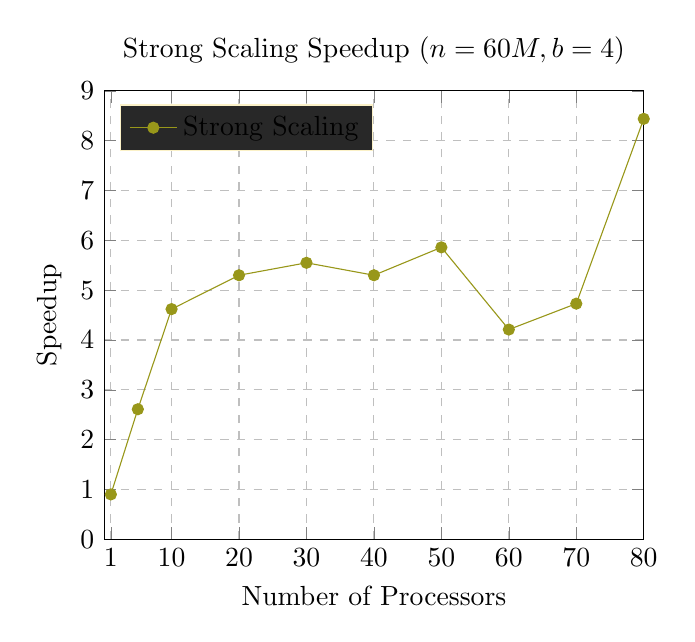
\begin{tikzpicture}
        \begin{axis}[
            title={Strong Scaling Speedup \( \left( n = 60M, b = 4 \right) \)},
            xlabel={Number of Processors},
            ylabel={Speedup},
            xmin=0, xmax=80,
            ymin=0, ymax=9,
            xtick={1,10,20,30,40,50,60,70,80},
            ytick={0,1,2,3,4,5,6,7,8,9},
            legend pos=north west,
            ymajorgrids=true,
            xmajorgrids=true,
            grid style=dashed,
            legend style={cells={anchor=west},fill=GBBackground,draw=GBForeground, legend pos=north west},
        ]

        \addplot[color=GBGreen,mark=*, mark options={fill=GBGreen}]
            coordinates {
                (1, 0.90) (5, 2.61) (10, 4.62) (20, 5.3) (30, 5.55)
                (40, 5.3) (50, 5.86) (60, 4.21) (70, 4.73) (80, 8.44)
            };
        \legend{Strong Scaling}
        \end{axis}
        \end{tikzpicture}
    \end{minipage}
    \hfill
    % Weak Scaling Plot
    \begin{minipage}{0.45\textwidth}
        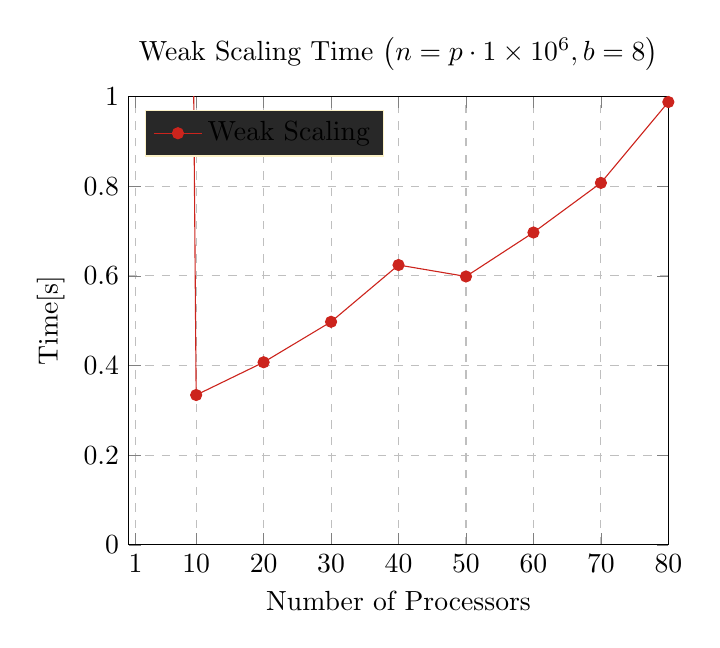
\begin{tikzpicture}
        \begin{axis}[
            title={Weak Scaling Time \( \left( n = p \cdot 1 \times 10^{6}, b = 8 \right) \)},
            xlabel={Number of Processors},
            ylabel={Time[s]},
            xmin=0, xmax=80,
            ymin=0, ymax=1,
            xtick={1,10,20,30,40,50,60,70,80},
            ytick={0,0.2,0.4,0.6,0.8,1},
            legend pos=north west,
            ymajorgrids=true,
            xmajorgrids=true,
            grid style=dashed,
            legend style={cells={anchor=west},fill=GBBackground,draw=GBForeground, legend pos=north west},
        ]

        \addplot[color=GBRed,mark=*, mark options={fill=GBRed}]
            coordinates {
                % (1, 0.258) (5, 0.375652) (10, 0.334089) (20, 0.407155)
                % (30, 0.497407) (40, 0.624086) (50, 0.598546) (60, 0.696600)
                % (70, 0.807231) (80, 0.987676)

                (1, 6.420776) (5, 9.615164) (10, 0.334089) (20, 0.407155)
                (30, 0.497407) (40, 0.624086) (50, 0.598546) (60, 0.696600)
                (70, 0.807231) (80, 0.987676)
            };
        \legend{Weak Scaling}
        \end{axis}
        \end{tikzpicture}
    \end{minipage}
\end{figure}

\subsection*{Weak Scaling}
\addcontentsline{toc}{subsection}{Weak Scaling}



\end{document}
